\documentclass[tikz,border=5pt]{standalone}
\usepackage[T1]{fontenc}
\usepackage[utf8]{inputenc}
\usepackage{lmodern}
\usepackage{amsmath,amssymb}
\usepackage{siunitx}
\usepackage{xcolor}
\usepackage{tikz}
\usetikzlibrary{
  arrows.meta,
  backgrounds,
  calc,
  decorations.pathreplacing,
  fit,
  matrix,
  positioning,
  shapes.geometric
}

\sisetup{
  detect-all = true,
  group-minimum-digits = 4,
}

\definecolor{TdcBlue}{HTML}{5B739F}
\definecolor{TdcRed}{HTML}{A35E66}
\definecolor{TdcLilac}{HTML}{8D83A7}
\definecolor{TdcCyan}{HTML}{82A9B8}
\definecolor{TdcGray}{HTML}{6D7175}
\definecolor{TdcBlack}{HTML}{202124}

\colorlet{TdcBlueFill}{TdcBlue!7}
\colorlet{TdcRedFill}{TdcRed!7}
\colorlet{TdcLilacFill}{TdcLilac!8}
\colorlet{TdcCyanFill}{TdcCyan!10}
\colorlet{TdcGrayFill}{black!3}
\colorlet{TdcGuide}{black!32}
\colorlet{TdcGuideLight}{black!18}

\tikzset{
  >=Latex,
  every picture/.style = {line join=round, line cap=round},
  every node/.style = {font=\small, text=TdcBlack},
  module/.style = {
    draw=black!72,
    fill=white,
    line width=0.50pt,
    rounded corners=0.8pt,
    minimum height=9mm,
    minimum width=22mm,
    align=center,
    inner sep=3pt
  },
  module gray/.style = {module, fill=TdcGrayFill},
  module slow/.style = {module, draw=TdcBlue, fill=TdcBlueFill},
  module fast/.style = {module, draw=TdcRed, fill=TdcRedFill},
  module ctrl/.style = {module, draw=TdcLilac, fill=TdcLilacFill},
  module io/.style = {module, draw=TdcCyan, fill=TdcCyanFill},
  domain box/.style = {
    draw=black!32,
    fill=black!1.5,
    line width=0.40pt,
    rounded corners=1.0pt,
    inner sep=4pt
  },
  domain label/.style = {
    font=\scriptsize\itshape,
    text=black!70
  },
  signal/.style = {-{Latex[length=2.2mm,width=1.5mm]}, draw=black!72, line width=0.60pt},
  signal slow/.style = {signal, draw=TdcBlue},
  signal fast/.style = {signal, draw=TdcRed},
  signal ctrl/.style = {signal, draw=TdcLilac},
  signal io/.style = {signal, draw=TdcCyan!80!black},
  signal dashed/.style = {signal, dashed},
  bidir/.style = {<->, draw=black!72, line width=0.55pt},
  guide/.style = {draw=TdcGuide, line width=0.35pt},
  guide dashed/.style = {guide, dashed},
  fine mark/.style = {draw=black!60, line width=0.40pt},
  brace note/.style = {
    decorate,
    decoration={brace, amplitude=3.0pt},
    draw=black!55,
    line width=0.40pt
  },
  note/.style = {
    font=\scriptsize,
    inner sep=1.5pt,
    fill=white,
    text=black!78
  },
  axis label/.style = {
    font=\scriptsize,
    text=black!72
  },
  lane label/.style = {
    font=\small,
    text=black!82
  },
  legend box/.style = {
    draw=black!60,
    line width=0.40pt,
    minimum width=4mm,
    minimum height=3mm
  },
  timeline block/.style = {
    draw=black!72,
    line width=0.45pt,
    minimum height=7.5mm,
    rounded corners=0.5pt,
    align=center,
    inner sep=2pt
  },
  timeline capture/.style = {timeline block, draw=TdcRed, fill=TdcRedFill},
  timeline snapshot/.style = {timeline block, draw=TdcLilac, fill=TdcLilacFill},
  timeline drain/.style = {timeline block, draw=TdcCyan!80!black, fill=TdcCyanFill},
  timeline free/.style = {timeline block, draw=black!60, fill=TdcGrayFill},
}

\newcommand{\DomainLabel}[2]{%
  \node[domain label, anchor=north west] at ($(#1.north west)+(0.10,-0.10)$) {#2};
}

\newcommand{\LegendItem}[4]{%
  \begin{scope}[shift={#1}]
    \node[legend box, fill=#2, anchor=west] at (0,0) {};
    \node[axis label, anchor=west] at (0.18,0) {#4};
  \end{scope}
}


\begin{document}
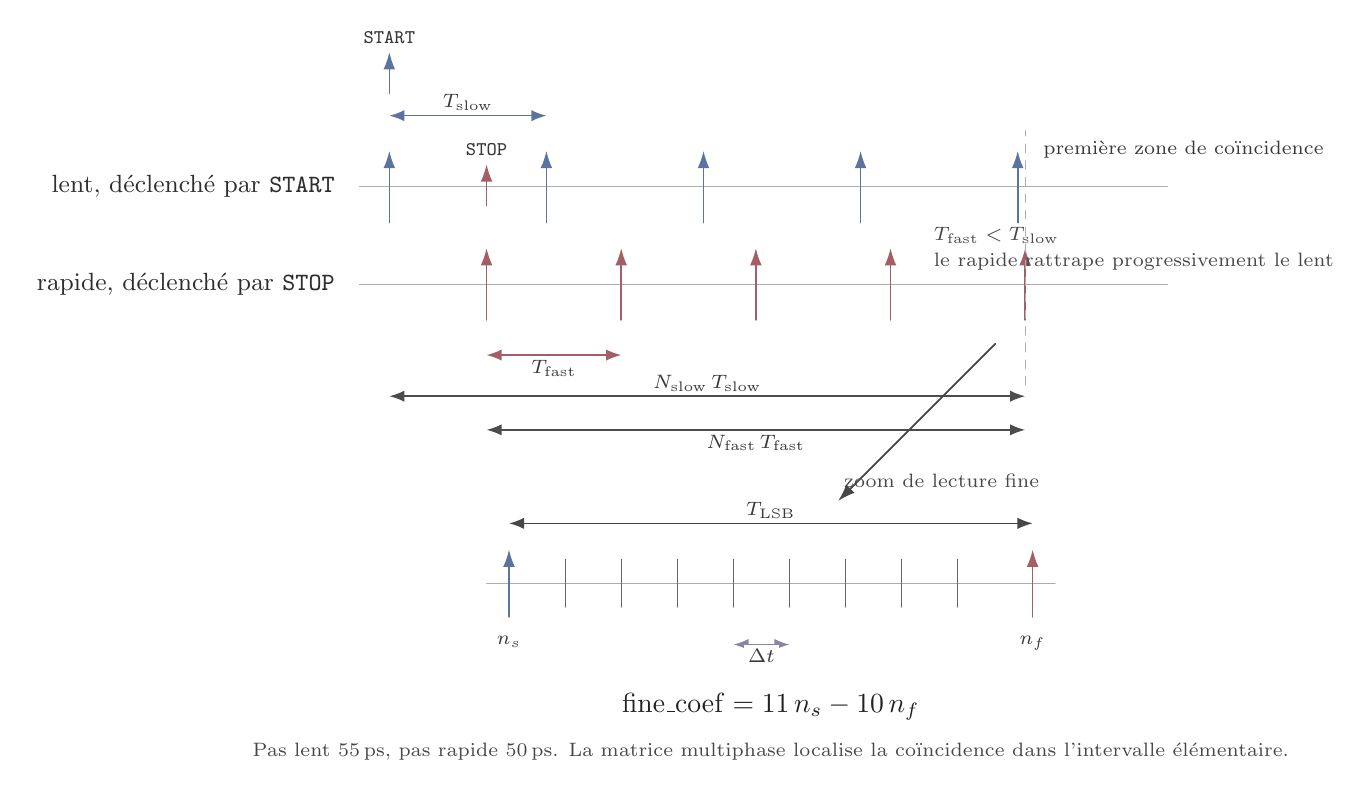
\begin{tikzpicture}[x=0.95cm,y=0.95cm]
  \coordinate (xmin) at (0.2,0);
  \coordinate (xmax) at (11.8,0);

  \draw[guide] (0.6,4.20) -- (11.4,4.20);
  \draw[guide] (0.6,2.90) -- (11.4,2.90);
  \node[lane label, anchor=east] at (0.40,4.20) {lent, déclenché par \texttt{START}};
  \node[lane label, anchor=east] at (0.40,2.90) {rapide, déclenché par \texttt{STOP}};

  \foreach \x in {1.0,3.1,5.2,7.3,9.4} {
    \draw[signal slow] (\x,3.72) -- (\x,4.68);
  }
  \foreach \x in {2.3,4.1,5.9,7.7,9.5} {
    \draw[signal fast] (\x,2.42) -- (\x,3.38);
  }

  \draw[guide dashed] (9.5,1.55) -- (9.5,4.95);
  \node[note, anchor=west] at (9.68,4.70) {première zone de coïncidence};

  \draw[signal slow] (1.0,5.45) -- ++(0,0.55);
  \node[note, above] at (1.0,6.05) {\texttt{START}};
  \draw[signal fast] (2.3,3.95) -- ++(0,0.55);
  \node[note, above] at (2.3,4.55) {\texttt{STOP}};

  \draw[bidir, draw=TdcBlue] (1.0,5.15) -- node[note, above] {$T_{\mathrm{slow}}$} (3.1,5.15);
  \draw[bidir, draw=TdcRed] (2.3,1.95) -- node[note, below] {$T_{\mathrm{fast}}$} (4.1,1.95);

  \draw[bidir, draw=black!70] (1.0,1.40) -- node[note, above] {$N_{\mathrm{slow}}\,T_{\mathrm{slow}}$} (9.5,1.40);
  \draw[bidir, draw=black!70] (2.3,0.95) -- node[note, below] {$N_{\mathrm{fast}}\,T_{\mathrm{fast}}$} (9.5,0.95);

  \node[axis label, anchor=west] at (8.15,3.55) {$T_{\mathrm{fast}} < T_{\mathrm{slow}}$};
  \node[axis label, anchor=west] at (8.15,3.20) {le rapide rattrape progressivement le lent};

  \draw[signal] (9.1,2.10) -- (7.0,0.00);
  \node[axis label, anchor=south west] at (6.95,0.05) {zoom de lecture fine};

  \draw[guide] (2.3,-1.10) -- (9.9,-1.10);
  \draw[signal slow] (2.6,-1.55) -- (2.6,-0.65);
  \draw[signal fast] (9.6,-1.55) -- (9.6,-0.65);
  \foreach \x in {3.35,4.10,4.85,5.60,6.35,7.10,7.85,8.60} {
    \draw[fine mark] (\x,-1.42) -- (\x,-0.78);
  }

  \draw[bidir, draw=black!72] (2.6,-0.30) -- node[note, above] {$T_{\mathrm{LSB}}$} (9.6,-0.30);
  \draw[bidir, draw=TdcLilac] (5.60,-1.92) -- node[note, below] {$\Delta t$} (6.35,-1.92);
  \node[note, anchor=north] at (2.6,-1.75) {$n_s$};
  \node[note, anchor=north] at (9.6,-1.75) {$n_f$};

  \node[font=\normalsize] at (6.1,-2.75) {$\mathrm{fine\_coef} = 11\,n_s - 10\,n_f$};
  \node[axis label, align=center] at (6.1,-3.35)
    {Pas lent \SI{55}{ps}, pas rapide \SI{50}{ps}. La matrice multiphase localise la coïncidence dans l'intervalle élémentaire.};
\end{tikzpicture}
\end{document}
